\chapter{Introduction}
Water is a fundamental molecule that plays an important role  in driving
numerous biological, chemical, environmental, and industrial processes. Water
is ubiquitous where it comprises two-thirds of earth and our own cells contain
two-thirds water by volume. Water is a unique molecule because it exists both
in
solid, liquid, and gas phase. Its ununsual properties include high boiling
point;
strong network of hydrogen bonds which directly correlates to  strong cohesion,
high surface
tension, heat of vaporization, and low vapor
pressure; ice has lower density than liquid water; and excellent solvent due to
its polar nature that
dissolve a wide range of substances, making it an excellent medium for chemical
reactions and biological processes \cite{Kontogeorgis2022}.

Due to its high cohesion, water can easily form surfaces and boundaries. Water
interfaces have important applications in heterogeneous catalysis, fuel cells,
and protein folding. In particular, aqueous solution containing salts affects
electrochemical gradients  that have important role in	cell membrane
regulation. Despite extensive research in both experimental and theoretical,
there exists a challenge in accurately modeling structural and dynamical
properties of salt solutions. An example is the role of chloride salts in
changing the surface tension of water as shown in
Figure~\ref{fig:surf_tens_solute}, where different trends are observed for
different chemical species.

Significant efforts were devoted to the development of models to reproduce the
behavior of water in computer simulations. The most
widely employed models for water are empirical models whose
parameters were obtained by fitting to experimentally measured properties. This
model is rigid and non transferrable. In contrast, ab initio models are
determined from first principles and
therefore do not require fitting to experimental data. However, this model is
computationally expensive and does not scale with large systems. Nevertheless,
recent advances in machine learning (ML) have allowed the development of Deep
neural network (DNN) potentials that
enables it to predict interfacial properties such as surface tension with the
same accuracy as the underlying ab-initio theory but as efficient as using
empirical methods.

This thesis will focus on the properties of a neat water (without any
solutes) in an interface and simulate relevant properties such as surface
tension, density, and dipole orientation using deep neural network potential
trained on bulk and with interfaces. Specifically, the objectives are

\begin{itemize}
    \item To develop accurate and transferrable DeepNN potentials for
          interfaces
    \item To explore the quality of the training data set in improving the
          description of water interfaces.
    \item To understand reliability of the current architecture of DeepMD in
          dealing with interfaces.
\end{itemize}

\begin{figure}[tbhp!]
    \centering
    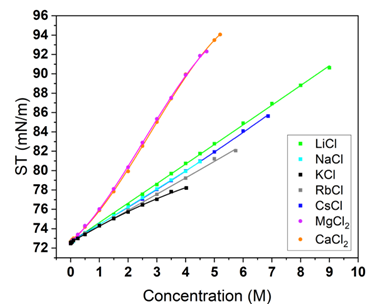
\includegraphics[width=0.75\linewidth]{images/ST_solute.png}
    \caption{Unpublished results from Paul Cremer's group at University of
        Pennsylvania  on surface tension measurements of chloride solutions.}
    \label{fig:surf_tens_solute}
\end{figure}